\RequirePackage{plautopatch}
\documentclass[upLaTeX,a4paper]{jsarticle}
\usepackage{listings,jlisting,amsmath,otf,here,empheq}
\usepackage[dvipdfmx]{graphicx}

\lstset{
breaklines = true,
numbers = left,
frame = tbrl,
tabsize = 4,
captionpos = t
}

\title{流体の数値計算プログラムの作成 レポート}
\author{B4 津田修一朗}
\date{2021/6/15}

\begin{document}
\maketitle

\section{環境}
プログラム実行環境: gfortran

グラフ描画ソフト: gnuplot

エディタ: Visual Studio Code

\section{数値計算の手順,手法}
\subsection{流れ関数と渦度を求めるプログラムの実装}
流れ関数-渦度法により,cavity内の流れを解いた.基礎方程式や境界条件については\cite{1}に従った.数値計算は,(i)レイノルズ数$Re = 50$, 格子点$50\times 50$, (ii)レイノルズ数$Re = 200$, 格子点$100\times 100$,
(iii) レイノルズ数$Re = 500$, 格子点$150\times 150$の3つの条件で行った.

\subsection{速度ベクトル図の描画}
流れ関数と渦度を求めるプログラムの実装により得られた流れ関数$\varPsi$より,速度場$(u, v)$を

\begin{equation}
  u = \frac{\partial \varPsi}{\partial y}, v = - \frac{\partial \varPsi}{\partial x},
\end{equation}
を用いて求めた.
ただし,u, vの境界条件は
\begin{empheq}{alignat=2}
  u = -1, v = 0 \quad 移動壁上 \\
  u = 0, v = 0 \quad 静止壁上
\end{empheq}
とした.

\subsection{流線図の描画}
流線は流れ関数$\varPsi = const$で表されることを用いて,流れ関数と渦度を求めるプログラムにより求めた流れ関数を用いて流線図を描画した.

\subsection{等圧線図の描画}
圧力のポアソン方程式
\begin{equation}
  \frac{\partial ^2 p}{\partial x ^2} + \frac{\partial ^2 p}{\partial y ^2} = 2 \left[ \left(\frac{\partial ^2 \varPsi}{\partial x ^2}\right) \left(\frac{\partial ^2 \varPsi}{\partial y ^2}\right) - \left( \frac{\partial ^2 \varPsi}{\partial x \partial y}  \right) ^2 \right]
\end{equation}
により圧力分布を求め,等圧線図を描画した.
差分方程式は
\begin{equation}
  \begin{split}
    p_{i,j}^{n+1} & =\frac{(p_{i+1,j}^{n}+p_{i-1,j}^{n})+(p_{i,j+1}^{n}+p_{i,j-1}^{n})-b_{i,j}^{n}h^2}{4}\\
    b_{i,j}^{n} & = 2\left[ \frac{\varPsi_{i+1,j}+\varPsi_{i-1,j}- 2\varPsi_{i,j}}{h^2} \frac{\varPsi_{i,j+1}+\varPsi_{i,j-1}-2\varPsi_{i,j}}{h^2} - \left(\frac{\varPsi_{i+1,j+1}-\varPsi_{i+1,j-1}-\varPsi_{i-1,j+1}+\varPsi_{i-1,j-1}}{4h^2}\right)^2  \right]
  \end{split}
\end{equation}
境界条件は
\begin{empheq}{alignat=2}
  \frac{\partial p}{\partial x} = 0 \quad (x=0, 1) \\
  \frac{\partial p}{\partial x} = 0 \quad (y=0,1)
\end{empheq}
とした.

\section{数値計算の結果}
\subsection{速度ベクトル図}
図1,2,3に今回得られた速度ベクトル図を示す.これらの図より,$(0,1),(1,1)$間を結ぶ線分に相当する移動壁面付近で比較的速い流れが生じ,cavity内に1つの渦ができていることが確認できる.
また,レイノルズ数$Re$が大きくなるにつれて、渦の中心が点(1, 1)に近づくことが確認できる.
さらに,レイノルズ数$Re=500$のときには$y=0$付近で流体の速さがおおよそ0であることがわかった.
\begin{figure}[H]
  \centering
  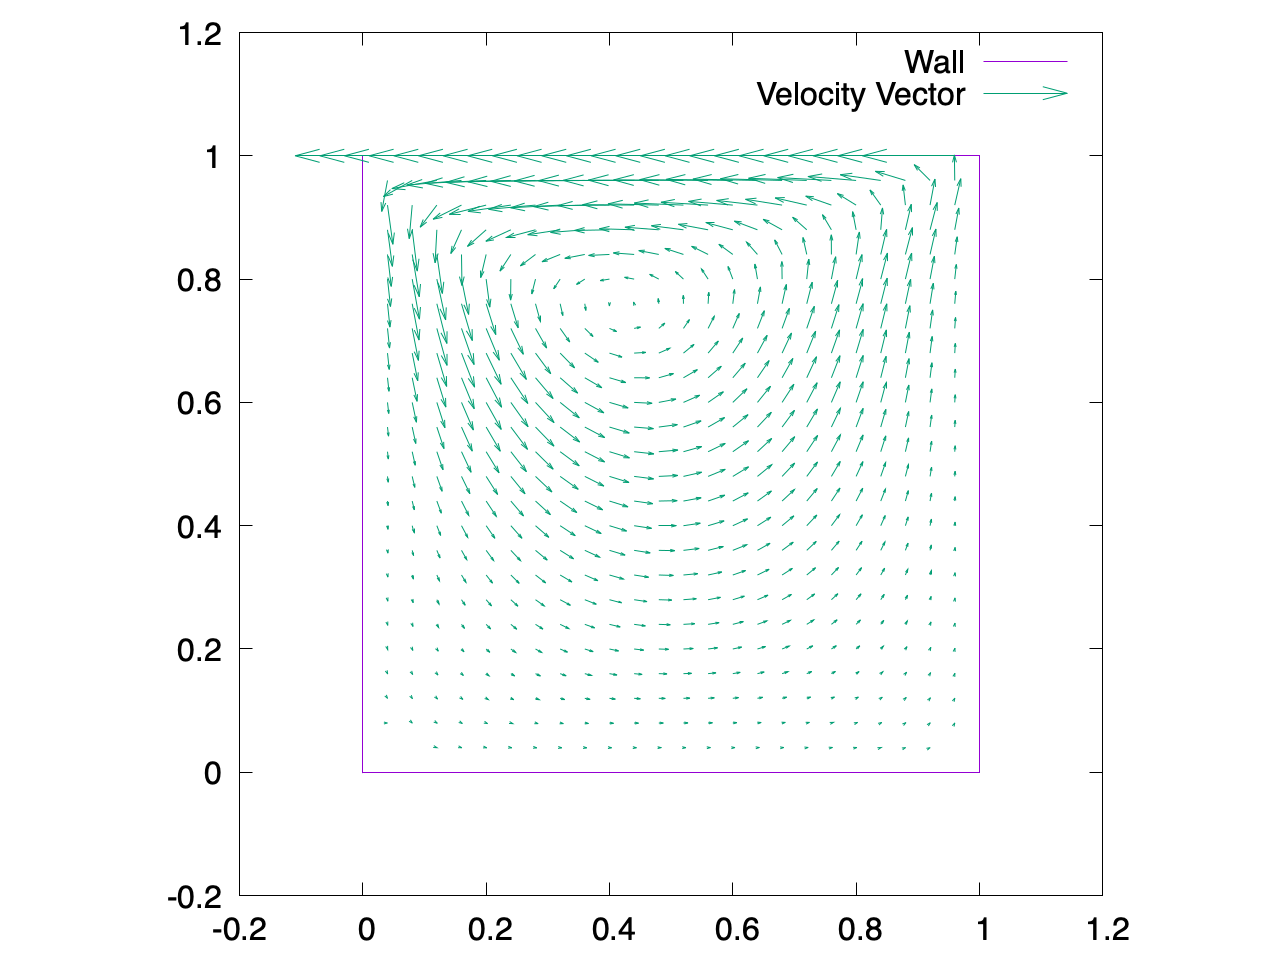
\includegraphics[height=9.5cm]{outputs/img/velocity_vector_re50.png}
  \caption{速度ベクトル図(i)}
  \label{fig:velocity_vector_re50}
\end{figure}
\begin{figure}[H]
  \centering
  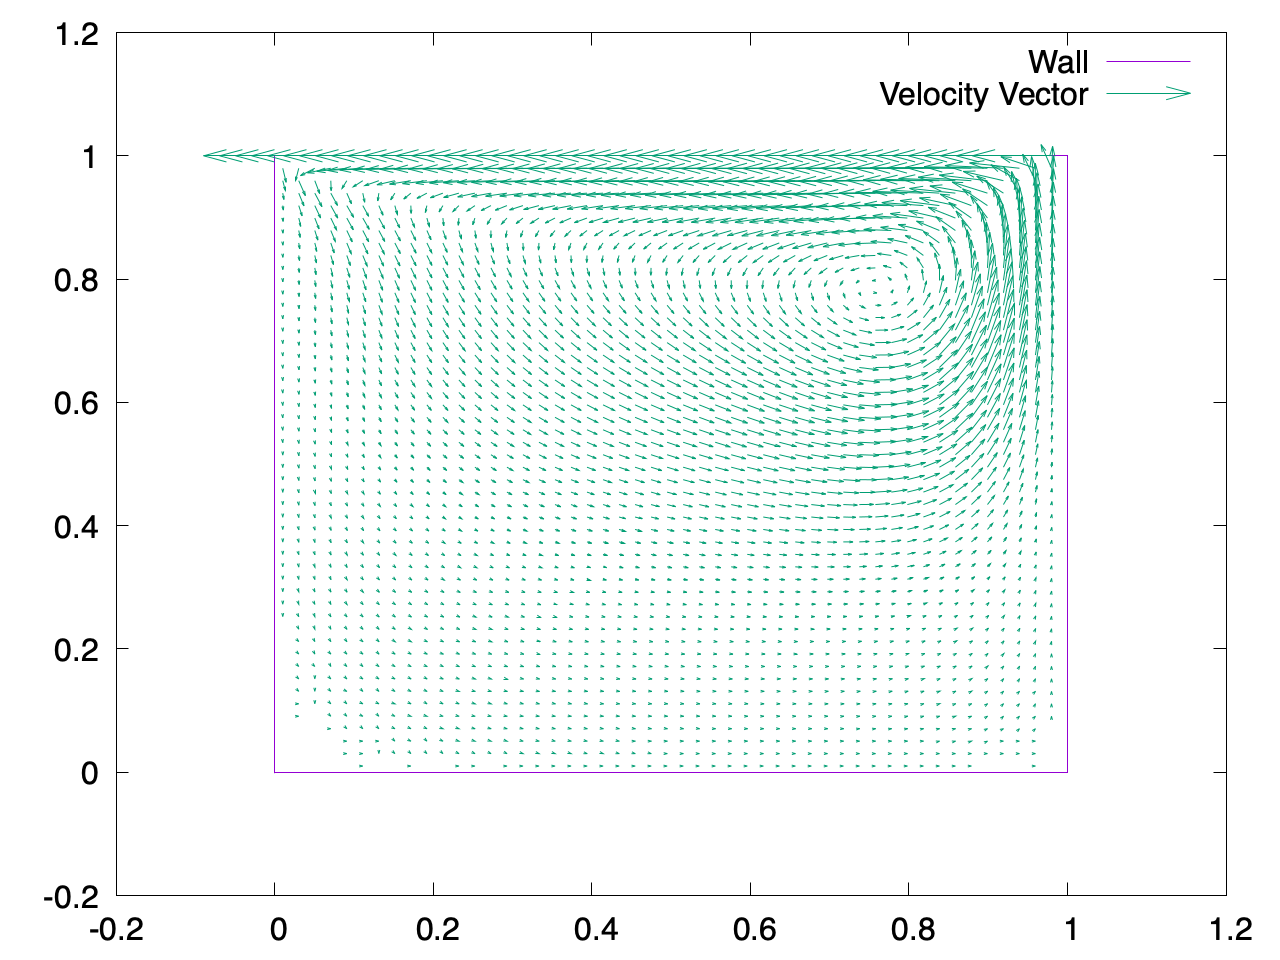
\includegraphics[height=9.5cm]{outputs/img/velocity_vector_re200.png}
  \caption{速度ベクトル図(ii)}
  \label{fig:velocity_vector_re200}
\end{figure}
\begin{figure}[H]
  \centering
  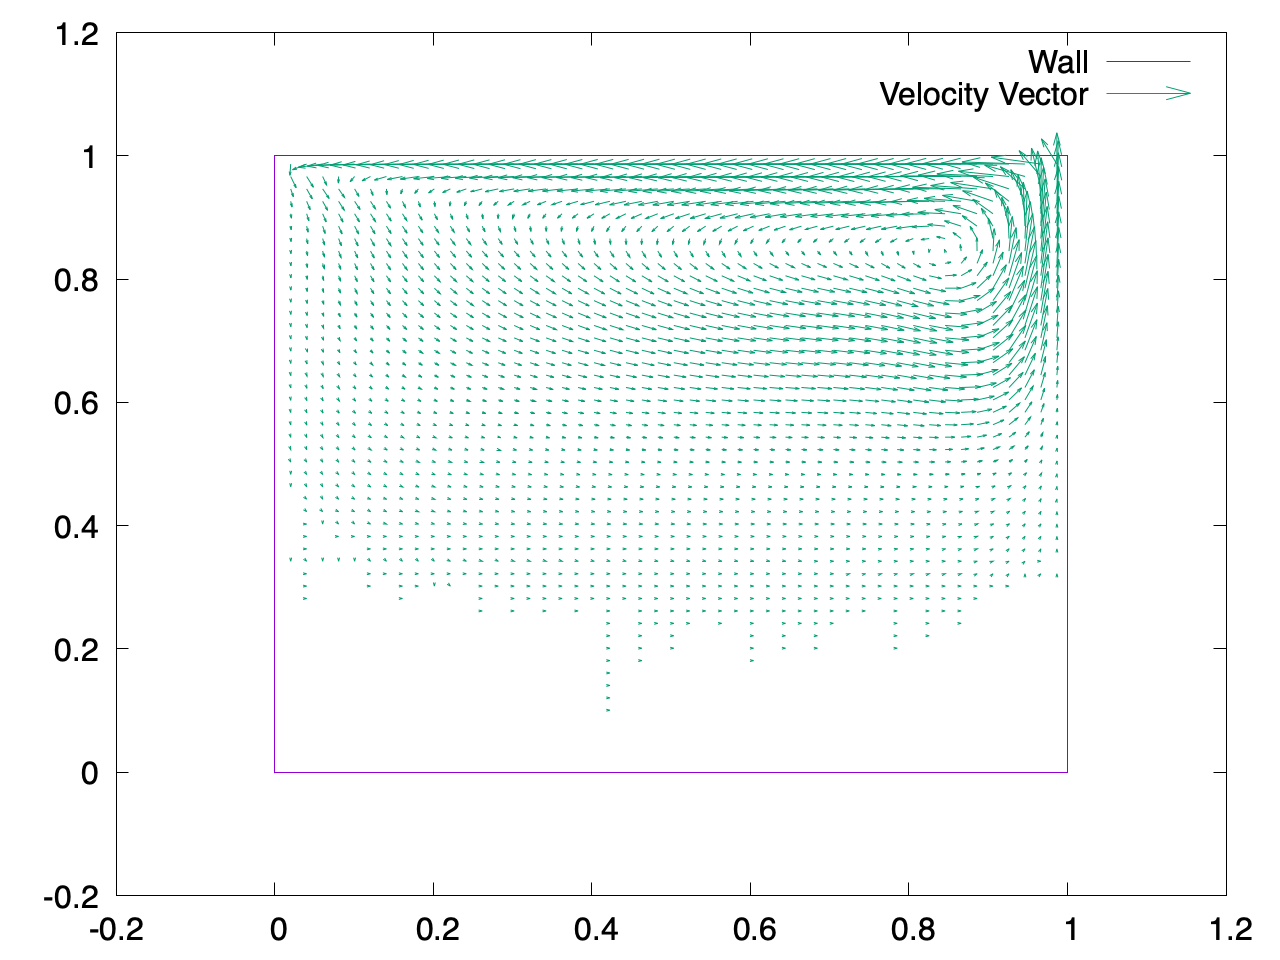
\includegraphics[height=9.5cm]{outputs/img/velocity_vector_re500.png}
  \caption{速度ベクトル図(iii)}
  \label{fig:velocity_vector_re500}
\end{figure}


\subsection{流線図}

図4,5,6に今回得られた流線図を示す.
中間報告においては, gnuplotの格子状データを生成するdgrid3d機能を用いていたため,比較的離れた格子点の情報が入ってしまっていた.
しかし,その後データを格納しているcsvファイルの形式を修正し,dgrid3dを使わず,数値解析によって得られた値をそのまま格子状データとして描画する方法を用いたので,最近接点のみの情報で表現できた.

\begin{figure}[H]
  \centering
  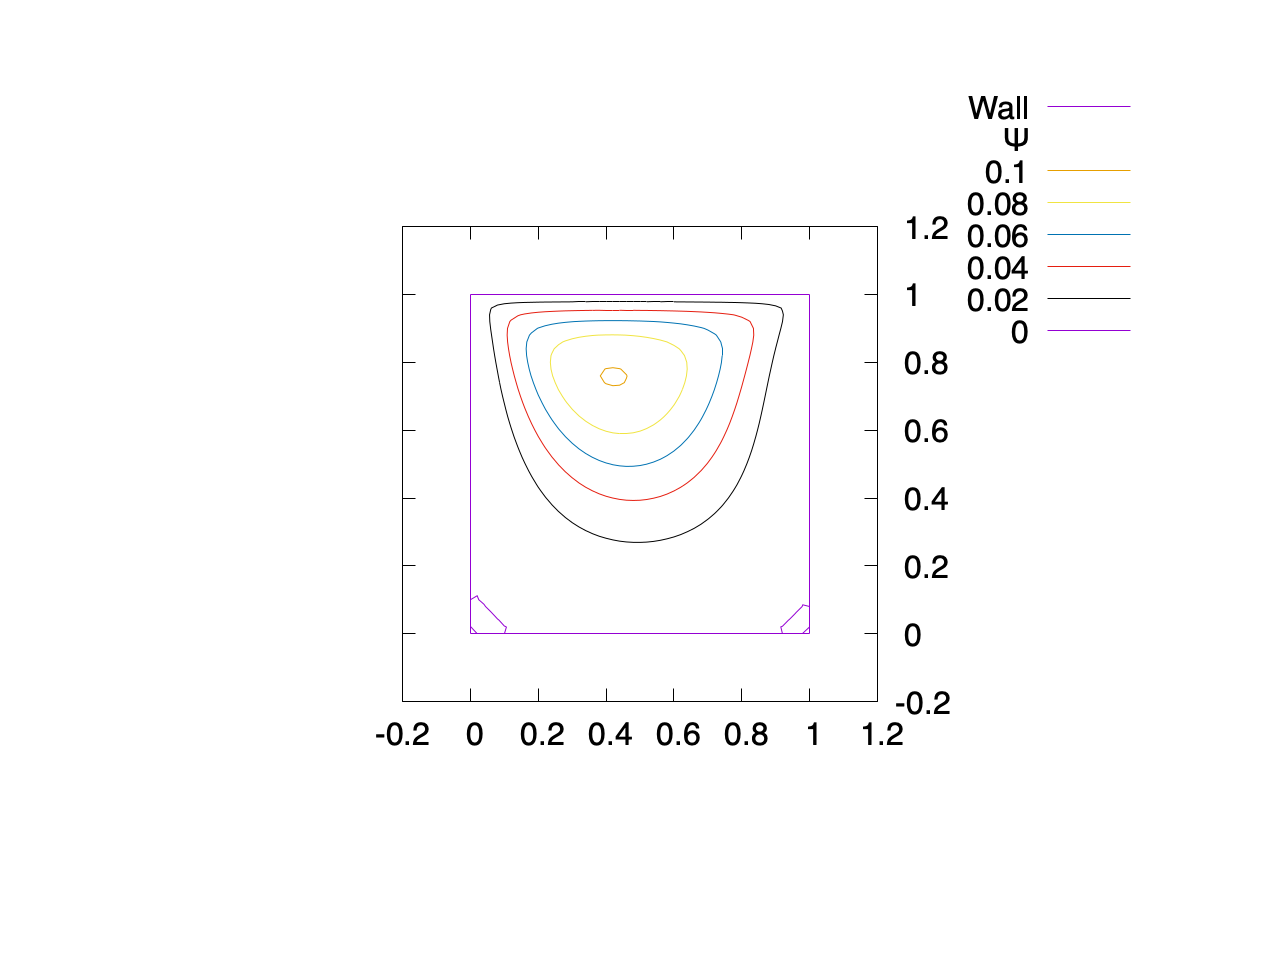
\includegraphics[height=9.5cm]{outputs/img/stream_line_re50.png}
  \caption{流線図(i)}
  \label{fig:velocity_vector_re50}
\end{figure}
\begin{figure}[H]
  \centering
  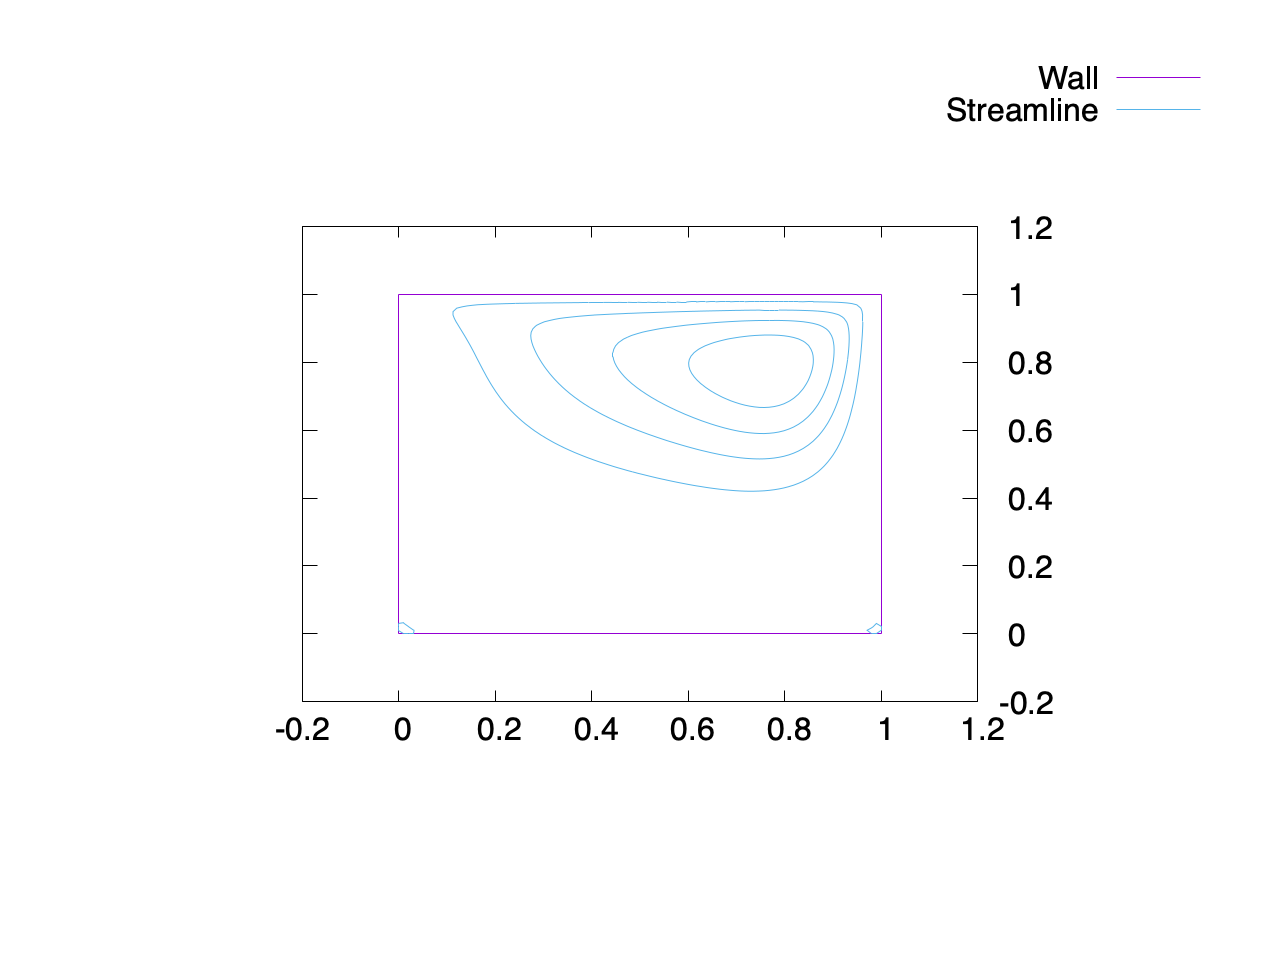
\includegraphics[height=9.5cm]{outputs/img/stream_line_re200.png}
  \caption{流線図(ii)}
  \label{fig:velocity_vector_re200}
\end{figure}
\begin{figure}[H]
  \centering
  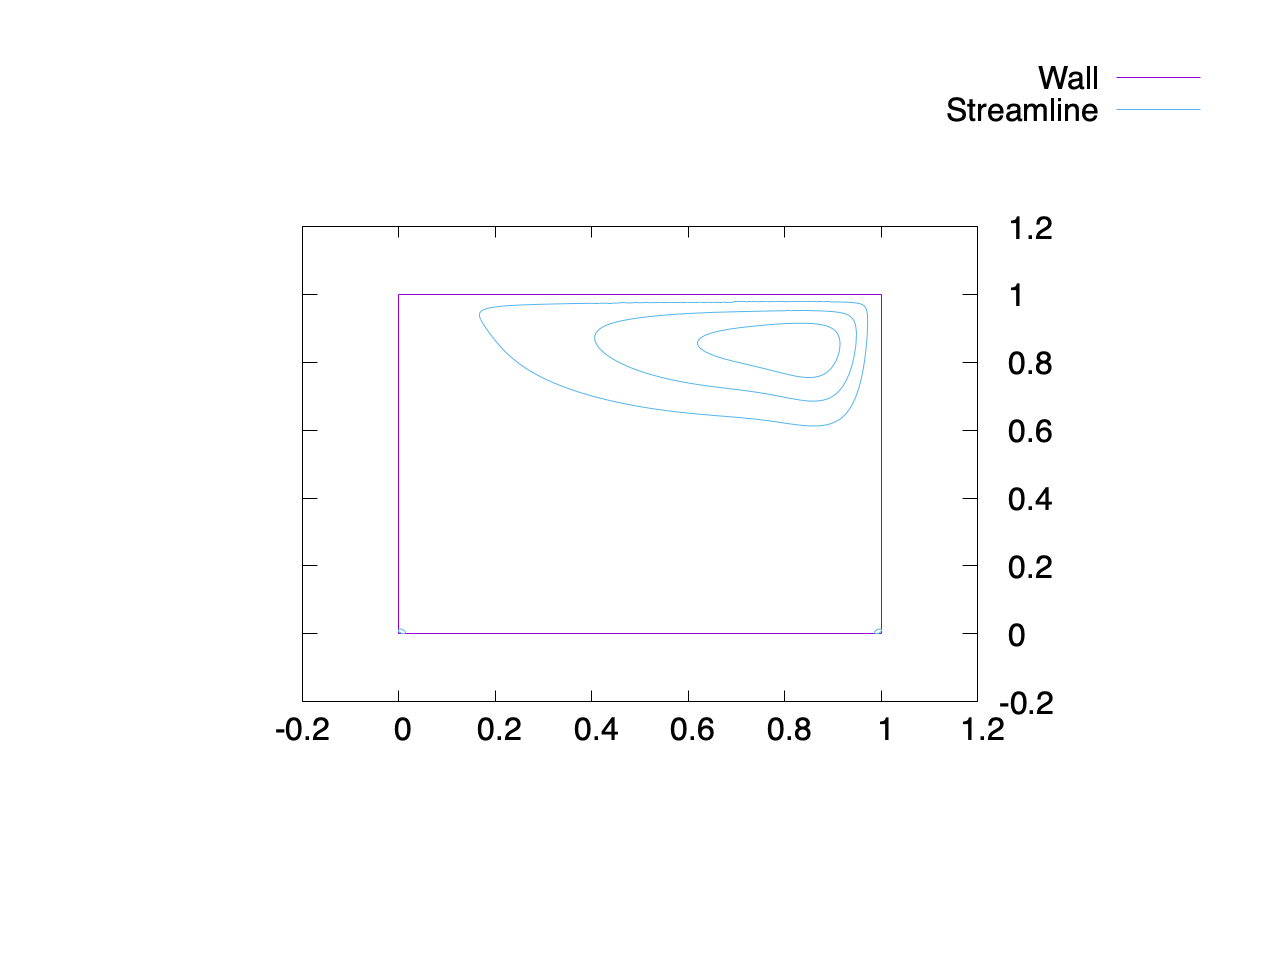
\includegraphics[height=9.5cm]{outputs/img/stream_line_re500.png}
  \caption{流線図(iii)}
  \label{fig:velocity_vector_re500}
\end{figure}


\subsection{等圧線図}
図7,8,9に今回得られた等圧線図を示す.
$(0,0),(1,0)$を結ぶ線分付近で圧力が高く,点(0,1),(1,1)付近で圧力が低い結果となった.
\begin{figure}[H]
  \centering
  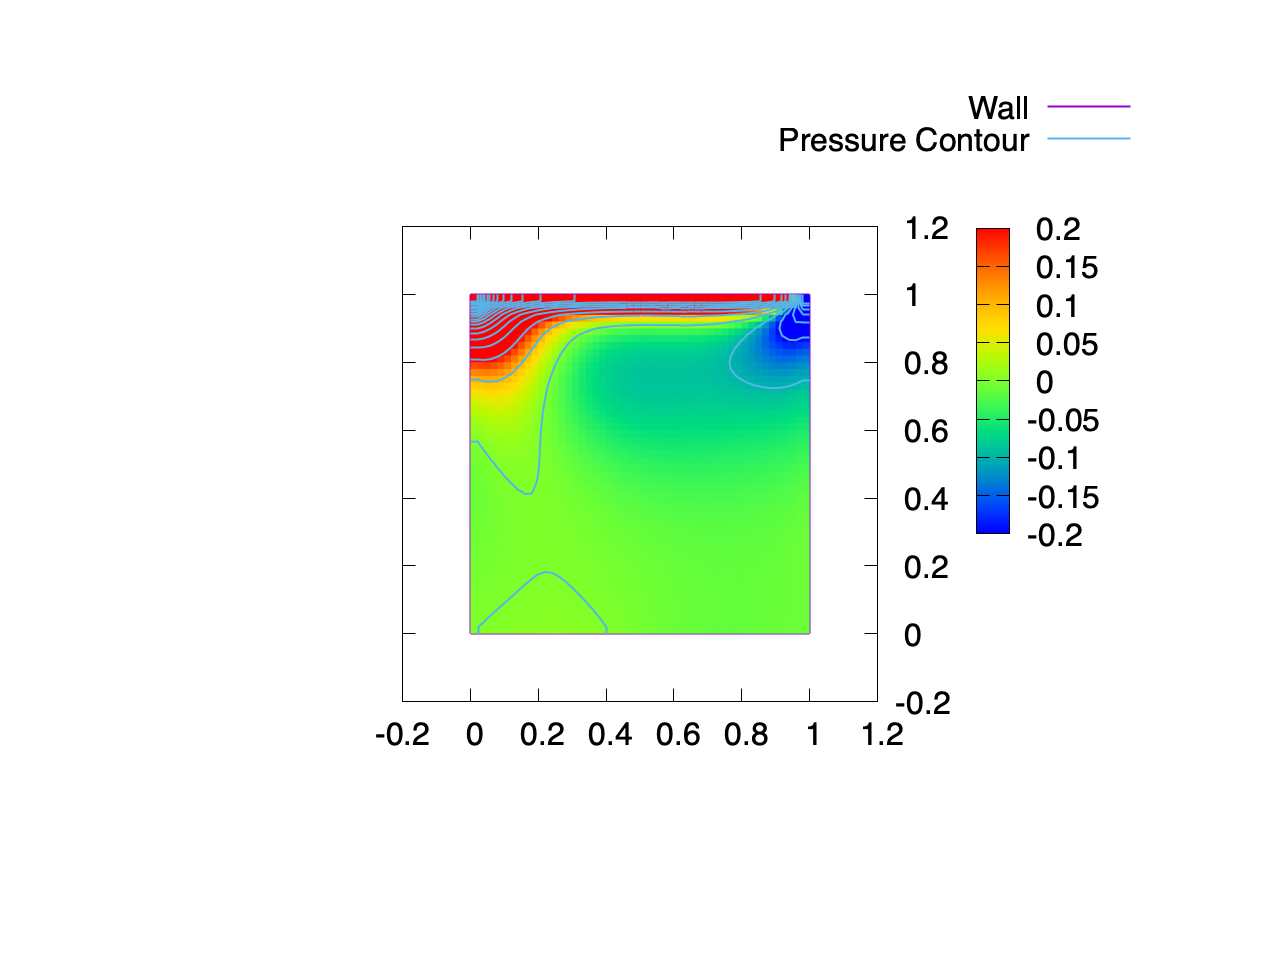
\includegraphics[height=9.5cm]{outputs/img/p_re50.png}
  \caption{等圧線図(i)}
  \label{fig:p_re50}
\end{figure}
\begin{figure}[H]
  \centering
  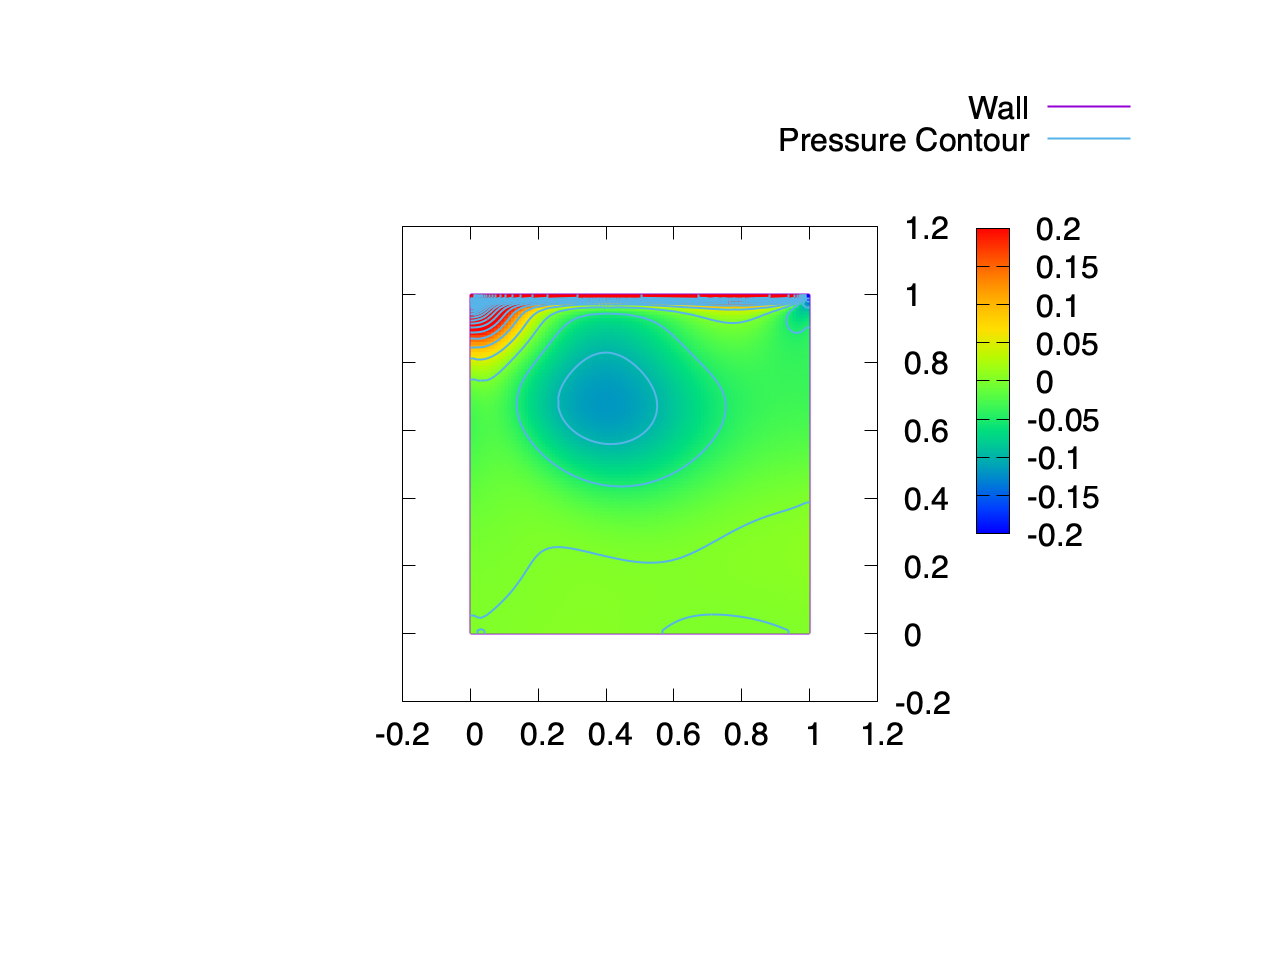
\includegraphics[height=9.5cm]{outputs/img/p_re200.png}
  \caption{等圧線図(ii)}
  \label{fig:p_re200}
\end{figure}
\begin{figure}[H]
  \centering
  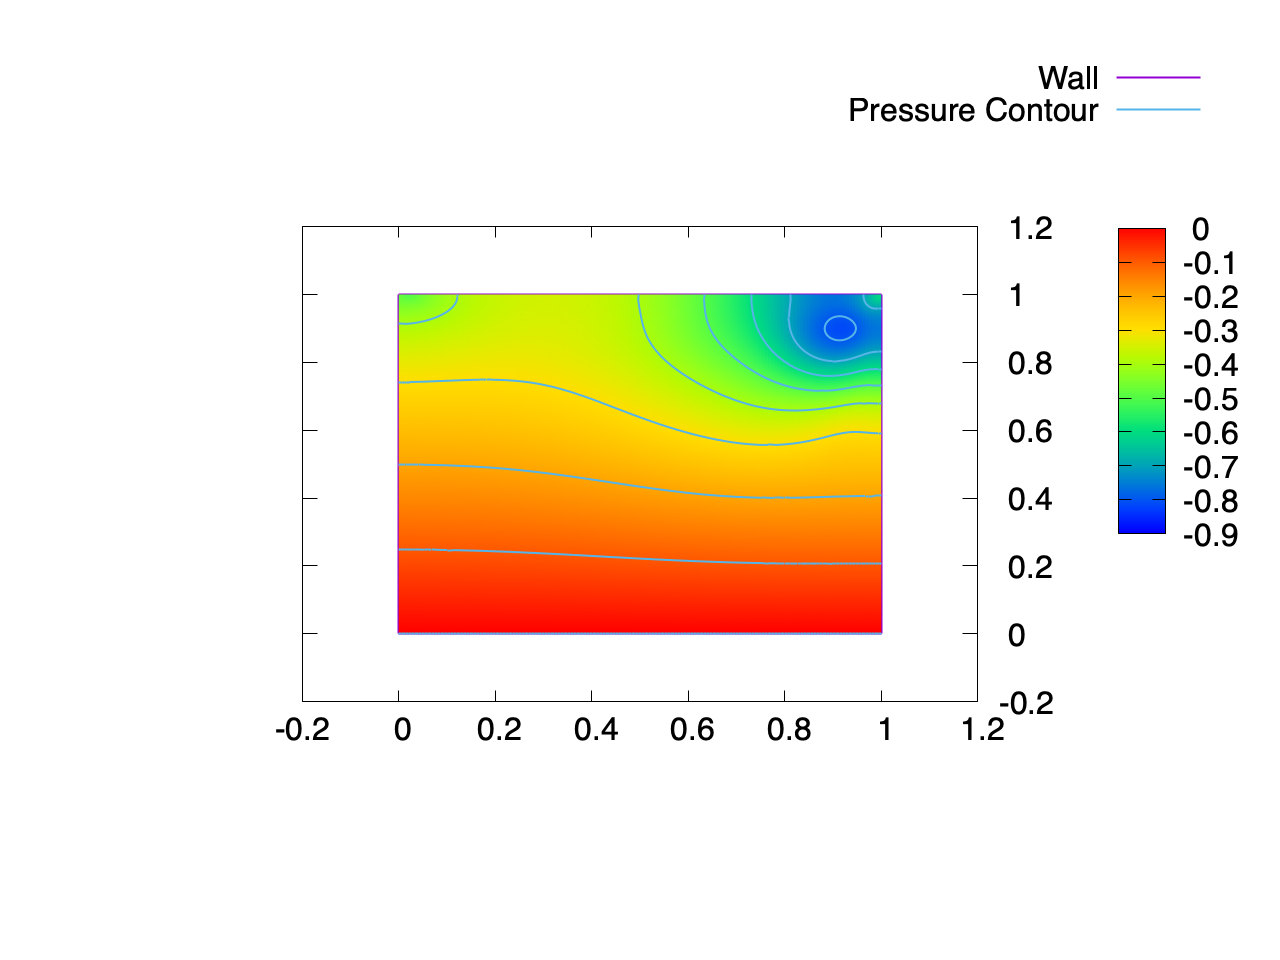
\includegraphics[height=9.5cm]{outputs/img/p_re500.png}
  \caption{等圧線図(iii)}
  \label{fig:p_re500}
\end{figure}

\begin{thebibliography}{9}
  %	\bibitem{1} \url{http://www.hal.t.u-tokyo.ac.jp/lab/ja/index_1.xhtml}
  %    \bibitem{2}Olga Russakovsky*, Jia Deng*, Hao Su, Jonathan Krause, Sanjeev Satheesh, Sean Ma, Zhiheng Huang, Andrej Karpathy, Aditya Khosla, Michael Bernstein, Alexander C. Berg and Li Fei-Fei. (* = equal contribution) ImageNet Large Scale Visual Recognition Challenge. IJCV, 2015.
  \bibitem{1} 研究室資料.流体の数値計算(川口光年先生1976年頃).pdf
\end{thebibliography}
\end{document}